%________________________________________________________________________________________________

\chapter{Preliminaries}
\label{chap:preliminaries}

Chapter~\ref{chap:intro} gave an informal overview of this thesis: it identified the verification problem, introduced local-timed negotiations informally, and stated the main decidability landscape. This chapter plays a different role. It fixes the formal background used in the rest of the thesis.

\section*{Why this chapter matters}
\begin{itemize}
    \item It introduces the two formal ingredients from which local-timed negotiations are built: \emph{negotiations} and \emph{timed automata}.
    \item It records the exact semantic notions that later proofs rely on: markings, guards, resets, regions, and reachability.
    \item It highlights one key contrast that drives the thesis: classical timed automata rely on \emph{global time}, whereas LTNs will use \emph{local time}.
\end{itemize}

\noindent No new results are proved in this chapter. Its purpose is to provide machinery, notation, and a shared reference point for later chapters.

\paragraph{Organization.}
Section~\ref{sec:prelim-negotiations} recalls negotiations as the control-flow model reused later. Section~\ref{sec:prelim-ta} recalls timed automata, now in full formal detail, because clocks, guards, resets, and regions are part of the later machinery. Section~\ref{sec:prelim-nta} reviews networks of timed automata only to isolate the global-time assumption from which LTNs depart. Section~\ref{sec:prelim-synthesis} states explicitly what Chapter~\ref{chap:ltn} will keep and what it will change. Section~\ref{sec:prelim-terminology} provides a compact terminology summary for quick reference in later chapters.

%________________________________________________________________________________________________

\section{Negotiations}
\label{sec:prelim-negotiations}

Negotiations provide the concurrency model underlying this thesis. Their defining feature is that \emph{multiparty interaction} is primitive: an atomic step is not a local transition of one component, but a joint interaction among all agents participating in a node. This makes both synchronization and independence visible in the model itself.

In the original formulation of Esparza and Desel~\cite{EsparzaDeselNegotiations}, outcomes may additionally update internal states of the participating agents through transformers. For the reachability questions studied in this thesis, those internal states are not essential. We therefore work with a control-flow presentation that records only which nodes each agent is ready to engage in next.

\subsection{Syntax and operational semantics}
\label{subsec:prelim-neg-syntax}

Let $P$ be a finite set of agents (or processes), and let $\Sigma$ be a finite set of outcome labels.

\begin{definition}[Negotiation]
\label{def:prelim-negotiation}
A \emph{negotiation} is a tuple
\[
\mathcal{N}=(N,\mathrm{dom},\mathrm{out},\delta)
\]
where:
\begin{itemize}
    \item $N$ is a finite set of nodes (also called \emph{atoms}),
    \item $\mathrm{dom} : N \to 2^P \setminus \{\emptyset\}$ assigns to each node a nonempty set of participating agents, called its \emph{domain},
    \item $\mathrm{out} : N \to 2^{\Sigma} \setminus \{\emptyset\}$ assigns to each node a nonempty finite set of \emph{available outcomes},
    \item for each agent $p \in P$, writing $N_p := \{n \in N : p \in \mathrm{dom}(n)\}$, we have a transition function
    \[
    \delta_p : \{(n,a) \in N_p \times \Sigma : a \in \mathrm{out}(n)\} \to 2^{N_p},
    \]
    where $\delta_p(n,a)$ is the set of nodes that agent $p$ becomes ready for after outcome $a$ occurs at node $n$.
\end{itemize}
We assume a distinguished initial node $n_{\mathrm{in}} \in N$ with $\mathrm{dom}(n_{\mathrm{in}})=P$.
\end{definition}

Thus, each node carries its own outcome set. The functions $\delta_p$ are total on the valid node--outcome pairs for agent $p$; there is no need to make them partial once $\mathrm{out}(n)$ is recorded explicitly.

A node $n$ with domain $\{p,q,r\}$ should be read as a point where agents $p,q,r$ must interact jointly. When the node occurs, they collectively choose one of the outcomes in $\mathrm{out}(n)$. The control effect of that outcome is described agent-by-agent by the functions $\delta_p$.

\begin{definition}[Marking]
A \emph{marking} is a function
\[
X : P \to 2^N
\]
with $X(p) \subseteq N_p$ for each $p \in P$. The intended meaning is that $X(p)$ is the set of nodes in which agent $p$ is currently ready to participate.
\end{definition}

The \emph{initial marking} $X_0$ is given by $X_0(p)=\{n_{\mathrm{in}}\}$ for every $p \in P$. We also use the \emph{final marking}
\[
X_f(p)=\emptyset \qquad \text{for all } p \in P,
\]
which represents termination. A node is enabled exactly when all of its participating agents are ready for it.

\begin{definition}[Enabled node and occurrence]
A node $n$ is \emph{enabled} at marking $X$ if $n \in X(p)$ for every $p \in \mathrm{dom}(n)$. If $n$ is enabled and the agents choose some outcome $a \in \mathrm{out}(n)$, the resulting marking $X'$ is defined by
\[
X'(p)=
\begin{cases}
\delta_p(n,a) & \text{if } p \in \mathrm{dom}(n),\\
X(p) & \text{if } p \notin \mathrm{dom}(n).
\end{cases}
\]
We write
\[
X \xrightarrow{(n,a)} X'
\]
and call this a \emph{small step}.
\end{definition}

A few points are worth emphasizing.
\begin{itemize}
    \item Readiness is \emph{replaced}, not accumulated. When an agent participates in an occurring node, its previous readiness set is discarded and replaced by the one prescribed by the chosen outcome.
    \item Synchronization is explicit. If two agents must move together, it is because they both belong to the domain of a node.
    \item Independence is also explicit. If two enabled nodes have disjoint domains, they may occur in either order.
\end{itemize}

\begin{definition}[Run, deadlock, livelock]
A \emph{run} of $\mathcal{N}$ is a finite or infinite sequence
\[
X_0 \xrightarrow{(n_1,a_1)} X_1 \xrightarrow{(n_2,a_2)} X_2 \xrightarrow{} \cdots .
\]
A finite run ending in $X_f$ is also called a \emph{large step}. A marking that enables no node is a \emph{deadlock}, unless it is the final marking $X_f$. A marking that can reoccur along an infinite run while the final marking remains unreachable is a \emph{livelock}.
\end{definition}

\begin{definition}[Reachability graph]
The \emph{reachability graph} of $\mathcal{N}$ has as vertices all markings reachable from $X_0$. There is an edge
\[
X \xrightarrow{(n,a)} X'
\]
whenever $X'$ is obtained from $X$ by one occurrence of $(n,a)$.
\end{definition}

This marking graph is the basic finite-state object associated with an untimed negotiation. In general it can be exponentially large in the size of the negotiation, and that blow-up is already visible before time is introduced.

\subsection{Graphical conventions}
\label{subsec:prelim-neg-graphics}

Negotiations admit a convenient graphical notation.
\begin{itemize}
    \item Each node is drawn as a thick black bar.
    \item For every participating agent, a white circle (a \emph{port}) is drawn on the bar.
    \item Outcome-labelled arrows leaving the ports describe the control flow of each participant after that outcome is chosen.
    \item If one outcome makes an agent ready for several possible next nodes, the edge branches as a \emph{hyperarc}.
    \item A marking is visualized by placing a token on the appropriate outgoing arc or branching point for each agent.
\end{itemize}

This representation is useful because it displays both causality and independence directly. Shared ports indicate enforced synchronization; disjoint ports indicate potential concurrency.

\subsection{A running example: ATM PIN reset}
\label{subsec:prelim-neg-atm}

We use a small ATM protocol as a running example throughout the preliminaries and later chapters. It is simple enough to read quickly, but rich enough to exhibit branching, retries, and multiparty interaction.

\paragraph{Scenario.}
A customer $c$ wants to reset their ATM PIN through an ATM machine $a$ and a bank $b$. The protocol proceeds as follows.
\begin{enumerate}
    \item All three agents first synchronize to start the transaction.
    \item The customer and the ATM interact to submit the request.
    \item The ATM and the bank interact to forward the details.
    \item The bank and the customer interact so that an OTP is sent.
    \item The customer re-enters the OTP through the ATM.
    \item The ATM and the bank validate the OTP; if the validation fails, the protocol returns to the OTP-entry stage.
    \item At a later attempt, the customer may instead give up; this makes the customer and the ATM ready for the completion node, while the bank continues according to its own current readiness.
\end{enumerate}

\paragraph{A fully explicit instance of Definition~\ref{def:prelim-negotiation}.}
Let
\[
P=\{c,a,b\}, \qquad N=\{n_{\mathrm{in}},n_1,n_2,n_3,n_4,n_5,n_6\},
\]
and let the global label alphabet be
\[
\Sigma=\{\mathsf{start},\mathsf{req},\mathsf{det},\mathsf{s\_otp},\mathsf{e\_otp},\mathsf{match},\mathsf{fail},\mathsf{g\_up},\mathsf{end}\}.
\]
The node domains are:
\[
\mathrm{dom}(n_{\mathrm{in}})=\{c,a,b\},\qquad \mathrm{dom}(n_1)=\{c,a\},\qquad \mathrm{dom}(n_2)=\{a,b\},
\]
\[
\mathrm{dom}(n_3)=\{c,b\},\qquad \mathrm{dom}(n_4)=\{c,a\},\qquad \mathrm{dom}(n_5)=\{a,b\},\qquad \mathrm{dom}(n_6)=\{c,a,b\}.
\]
The node-wise outcome sets are:
\[
\mathrm{out}(n_{\mathrm{in}})=\{\mathsf{start}\},\quad \mathrm{out}(n_1)=\{\mathsf{req}\},\quad \mathrm{out}(n_2)=\{\mathsf{det}\},\quad \mathrm{out}(n_3)=\{\mathsf{s\_otp}\},
\]
\[
\mathrm{out}(n_4)=\{\mathsf{e\_otp},\mathsf{g\_up}\},\quad \mathrm{out}(n_5)=\{\mathsf{match},\mathsf{fail}\},\quad \mathrm{out}(n_6)=\{\mathsf{end}\}.
\]
Writing $N_c=\{n_{\mathrm{in}},n_1,n_3,n_4,n_6\}$, $N_a=\{n_{\mathrm{in}},n_1,n_2,n_4,n_5,n_6\}$, and $N_b=\{n_{\mathrm{in}},n_2,n_3,n_5,n_6\}$, the actually defined transition values are:

\medskip
\noindent\textbf{Customer $c$.}
\[
\delta_c(n_{\mathrm{in}},\mathsf{start})=\{n_1\}, \qquad
\delta_c(n_1,\mathsf{req})=\{n_3\}, \qquad
\delta_c(n_3,\mathsf{s\_otp})=\{n_4\},
\]
\[
\delta_c(n_4,\mathsf{e\_otp})=\{n_4,n_6\}, \qquad
\delta_c(n_4,\mathsf{g\_up})=\{n_6\}, \qquad
\delta_c(n_6,\mathsf{end})=\emptyset.
\]

\noindent\textbf{ATM $a$.}
\[
\delta_a(n_{\mathrm{in}},\mathsf{start})=\{n_1\}, \qquad
\delta_a(n_1,\mathsf{req})=\{n_2\}, \qquad
\delta_a(n_2,\mathsf{det})=\{n_4\},
\]
\[
\delta_a(n_4,\mathsf{e\_otp})=\{n_5\}, \qquad
\delta_a(n_4,\mathsf{g\_up})=\{n_6\}, \qquad
\delta_a(n_5,\mathsf{match})=\{n_6\},
\]
\[
\delta_a(n_5,\mathsf{fail})=\{n_4\}, \qquad
\delta_a(n_6,\mathsf{end})=\emptyset.
\]

\noindent\textbf{Bank $b$.}
\[
\delta_b(n_{\mathrm{in}},\mathsf{start})=\{n_2\}, \qquad
\delta_b(n_2,\mathsf{det})=\{n_3\}, \qquad
\delta_b(n_3,\mathsf{s\_otp})=\{n_5\},
\]
\[
\delta_b(n_5,\mathsf{match})=\{n_6\}, \qquad
\delta_b(n_5,\mathsf{fail})=\{n_5\}, \qquad
\delta_b(n_6,\mathsf{end})=\emptyset.
\]
No other values of $\delta_c$, $\delta_a$, or $\delta_b$ are in the domain of the corresponding function, because outcomes are only defined at nodes whose outcome sets contain them.

\paragraph{How the control flow works.}
From the initial marking $X_0$, outcome $\mathsf{start}$ sends $c$ and $a$ to $n_1$ and sends $b$ to $n_2$. After the request step at $n_1$, the ATM moves to $n_2$, enabling the ATM--bank interaction that forwards the request to the bank. The OTP is then sent at $n_3$, the customer re-enters it at $n_4$, and validation occurs at $n_5$. Outcome $\mathsf{fail}$ returns the ATM to $n_4$ and keeps the bank at $n_5$, thereby creating the retry pattern. Outcome $\mathsf{g\_up}$ at $n_4$ makes the customer and the ATM ready for $n_6$; whether $n_6$ then becomes enabled depends on where the bank currently is in the protocol.

\paragraph{Why this example matters later.}
This example will reappear in Chapter~\ref{chap:ltn} once clocks are added. It is particularly convenient there because the untimed control structure is already familiar, so one can isolate what is genuinely new about the local-time semantics.

Figure~\ref{fig:ATM} shows the graphical representation of this negotiation.

\begin{figure}[t]
\centering
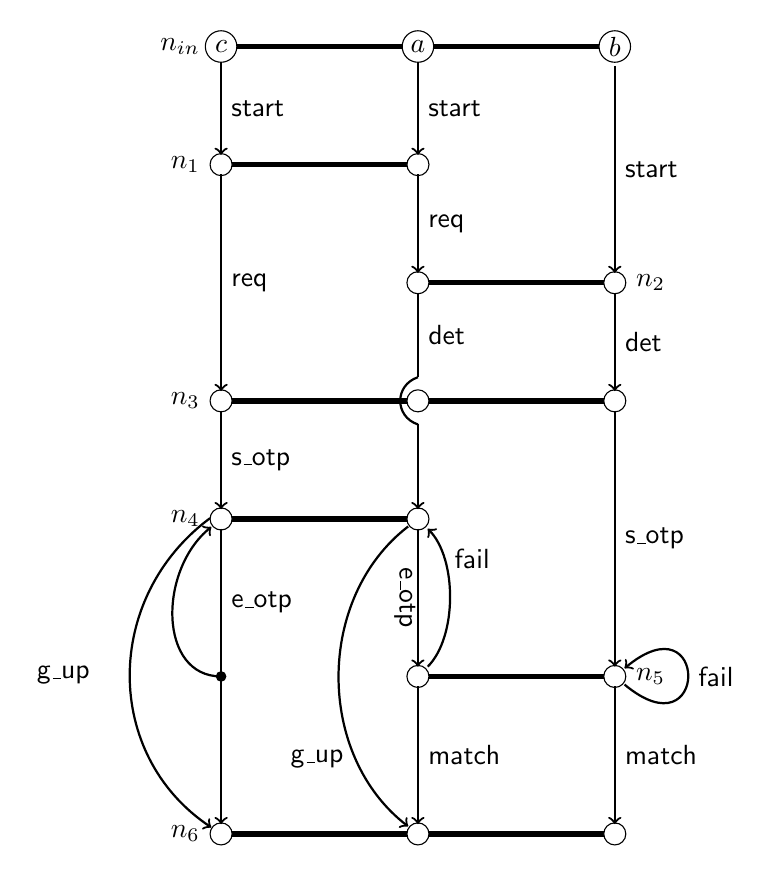
\begin{tikzpicture}

\begin{scope}[line width=2pt]
\draw (0.,0) node [left] {$n_{\text{in}}\,\,$} -- (5,0);
\draw (0.,-1.5) node [left] {$n_{1}\,\,$} -- (2.5,-1.5);
\draw (2.5,-3) -- (5,-3) node [right] {$\,\,n_{2}$};
\draw (0.,-4.5) node [left] {$n_{3}\,\,$} -- (5,-4.5);
\draw (0.,-6) node [left] {$n_{4}\,\,$} -- (2.5,-6);
\draw (2.5,-8) -- (5,-8)  node [right] {\,\,$n_{5}$};
\draw (0.,-10) node [left] {$n_{6}\,\,$} -- (5,-10);
\end{scope}

\begin{scope}[fill=white]
\filldraw  (0,0)  circle (2mm) node (nic) {$c$};
\filldraw  (2.5,0)  circle (2mm) node (nia) {$a$};
\filldraw  (5,0)  circle (2mm) node (nib) {$b$};

\filldraw  (0,-1.5)  circle (1.4mm) node (n1c) {};
\filldraw  (2.5,-1.5)  circle (1.4mm) node (n1a) {};

\filldraw  (2.5,-3)  circle (1.4mm) node (n2a) {};
\filldraw  (5,-3)  circle (1.4mm) node (n2b) {};

\filldraw  (0,-4.5)  circle (1.4mm) node (n3c) {};
\filldraw  (2.5,-4.5)  circle (1.4mm) node (n3a) {};
\filldraw  (5,-4.5)  circle (1.4mm) node (n3b) {};

\filldraw  (0,-6)  circle (1.4mm) node (n4c) {};
\filldraw  (2.5,-6)  circle (1.4mm) node (n4a) {};

\filldraw  (2.5,-8)  circle (1.4mm) node (n5a) {};
\filldraw  (5,-8)  circle (1.4mm) node (n5b) {};

\filldraw  (0,-10)  circle (1.4mm) node (n6c) {};
\filldraw  (2.5,-10)  circle (1.4mm) node (n6a) {};
\filldraw  (5,-10)  circle (1.4mm) node (n6b) {};

\filldraw  [fill=black] (0,-8)  circle (0.6mm) node (v1) {};
\end{scope}

\begin{scope}[thick,->]
\draw (nic) -- (n1c) node [right, midway] {$\mathsf{start}$};
\draw (n1c) -- (n3c) node [right, midway] {$\mathsf{req}$};
\draw (n3c) -- (n4c) node [right, midway] {$\mathsf{s\_otp}$};
\draw (n4c) -- (n6c) node [right, text width = 1.5 cm, near start] {$\mathsf{e\_otp}$};
\draw (0,-8) .. controls  (-0.8,-8) and (-0.8,-6.65) .. (n4c) node [left, midway] {};

\draw (nia) -- (n1a) node [right, midway] {$\mathsf{start}$};
\draw (n1a) -- (n2a) node [right, midway] {$\mathsf{req}$};
\draw (2.5,-4.8) -- (n4a);
\draw (n4a) -- (n5a) node [below=-0.1cm, sloped, midway] {$\mathsf{e\_otp}$};
\draw (n5a) -- (n6a) node [right, text width = 1 cm, midway] {$\mathsf{match}$};
\draw (n5a) .. controls (3,-7.5) and (3,-6.5) .. (n4a) node [right, near end] {$\mathsf{fail}$};
\draw (n4a) .. controls  (1.2,-7) and (1.2,-9) .. (n6a) node [left=-0.3cm, text width = 1 cm, near end] {$\mathsf{g\_up}$};

\draw (nib) -- (n2b) node [right, midway] {$\mathsf{start}$};
\draw (n2b) -- (n3b) node [right, midway] {$\mathsf{det}$};
\draw (n3b) -- (n5b) node [right, text width = 1 cm, midway] {$\mathsf{s\_otp}$};
\draw (n5b) -- (n6b) node [right, text width = 1 cm, midway] {$\mathsf{match}$};
\draw (n5b) .. controls  (6.2,-9) and (6.2,-7) .. (n5b) node [right, midway] {$\mathsf{fail}$};

\draw (n4c) + (-0.14,0.01) .. controls  (-1.5,-7) and (-1.5,-9) .. (n6c) node [left=-0.2cm, text width = 1.25 cm, midway] {$\mathsf{g\_up}$};
\end{scope}

\draw [thick] (n2a) -- (2.5,-4.2) node [right, midway] {$\mathsf{det}$};
\draw [thick] (2.5,-4.2) .. controls (2.2,-4.3) and (2.2,-4.7) .. (2.5,-4.8);
\end{tikzpicture}
\caption{ATM transaction negotiation. Customer ($c$), ATM ($a$), and bank ($b$) coordinate through atomic interactions. Note the hyperarc at $n_4$ for customer $c$ after $\mathsf{e\_otp}$: non-deterministic control flow allows readiness at both $n_4$ (retry) and $n_6$ (completion).}
\label{fig:ATM}
\end{figure}

\subsection{A richer example: pollination and climate mismatch}
\label{subsec:prelim-neg-pollination}

The ATM protocol is useful as a running workflow example, but it is mostly a
structured coordination pattern with one main retry loop. For branching,
hyperarcs, delayed resolution of choice, and possible blow-up of the marking
graph, it is helpful to keep a second, more visibly nondeterministic example in
view.

Consider a stylized negotiation inspired by the mismatch between flowering time
and pollinator emergence. Let the agents be
\[
P=\{t,e,b\},
\]
where $t$ stands for \emph{trees}, $e$ for the \emph{environment}, and $b$ for
\emph{bees}. The point of the example is not ecological realism, but a compact
interaction pattern in which several local choices jointly determine what can
happen later.

\paragraph{Informal reading.}
The trees, the environment, and the bees first evolve separately. Trees may move
through a seasonal-change step, the environment may choose between a ``good
climate'' and a ``climate change'' branch, and bees may move through an
emergence step. Later, trees and the environment interact to determine whether
flowering is normal or early. Finally, the system returns to the beginning of a
new cycle. The example is useful because the consequences of earlier choices are
not resolved immediately: they constrain which later multiparty interactions can
become enabled.

\paragraph{Key observations from this example.}
This example illustrates several features of negotiations:
\begin{enumerate}
\item \textbf{Multiparty interactions are atomic:} An interaction involves all its participating agents simultaneously and cannot be decomposed into pairwise steps. Node \(n_6\) requires all three processes to participate simultaneously.
\item \textbf{Synchronization is explicit, not emergent:} Agents synchronize because the model says so, not because of shared state.
\item \textbf{Independence is visible in the structure:} Disjoint sets of agents can proceed independently, and this is evident in the graph itself. Nodes \(n_1\), \(n_2\) and \(n_3\) can occur in either order, or even conceptually ``at the same time'' since they involve disjoint sets of processes.
\item \textbf{Non-determinism:} After \(n_1\), \(t\) is ready to engage in both \(n_4\) and \(n_5\) and the choice is resolved only through interaction.
\item \textbf{Control flow is global, not agent-local:} Choices made at one node propagate to future possibilities for all involved agents.
\item \textbf{Information transfer:} The example highlights that synchronization itself acts as a mechanism for
information flow between agents -- by participating in a joint interaction, agents
implicitly exchange information that influences future behavior, even though no
explicit shared state or data is modeled.
\item \textbf{Succicntness:} The underlying reachability graph could be exponential on the number of nodes.
\end{enumerate}

Figure~\ref{fig:prelim-pollination} gives the negotiation graph. A sample run and
an excerpt of the corresponding reachability graph are deferred to
Appendix~\ref{app:pollination-extended} so that the main text can keep the focus
on the formal machinery.

In general, occurrence sequences can be arbitrarily long, and the number of reachable markings can be very large. For negotiations with multiple hyperarcs, each with branching degree \(n\), the number of distinct branching patterns can grow as \(n^k\), where \(k\) is the number of hyperarcs, leading to an exponential blow-up in the marking graph. It is known that the reachability problem for negotiations is PSPACE-complete in general, and already coNP-hard and in DP for acyclic negotiations (see, e.g.,~\cite{EsparzaDeselNegotiations}).

\begin{figure}[t]
\centering
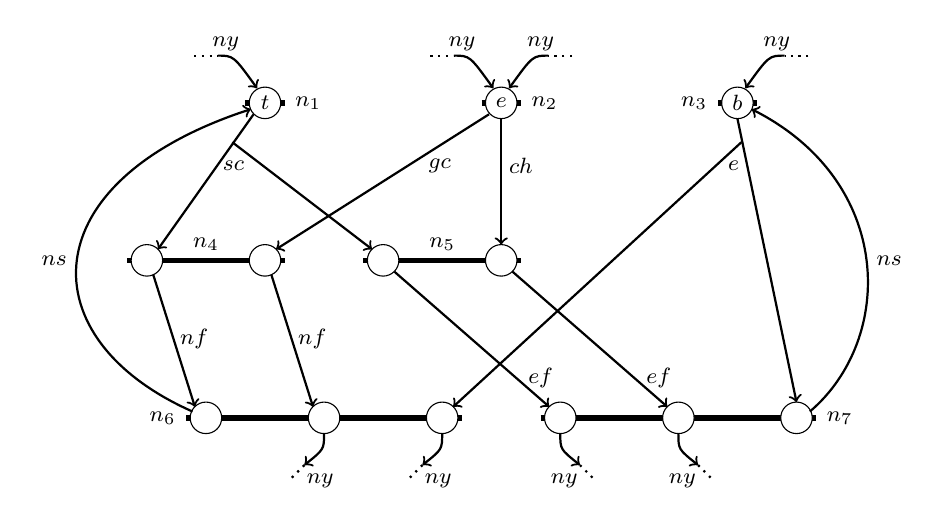
\begin{tikzpicture}[scale=1, every node/.style={transform shape}]

\begin{scope}[line width=2pt]
\draw (-0.25,0) -- (0.25,0);
\draw (2.75,0) -- (3.25,0);
\draw (5.75,0) -- (6.25,0);
\draw (-1.75,-2) -- (0.25,-2);
\draw (1.25,-2) -- (3.25,-2);
\draw (-1,-4) -- (2.5,-4);
\draw (3.5,-4) -- (7,-4);
\end{scope}

\filldraw [fill=white]  (0,0)  circle (2mm) node (t0) {\footnotesize $t$};
\filldraw [fill=white]  (3,0)  circle (2mm) node (e0) {\footnotesize $e$};
\filldraw [fill=white]  (6,0)  circle (2mm) node (b0) {\footnotesize $b$};
\filldraw [fill=white]  (-1.5,-2)  circle (2mm) node (t1) {};
\filldraw [fill=white]  (0,-2)  circle (2mm) node (e1) {};
\filldraw [fill=white]  (1.5,-2)  circle (2mm) node (t2) {};
\filldraw [fill=white]  (3,-2)  circle (2mm) node (e2) {};
\filldraw [fill=white]  (-0.75,-4)  circle (2mm) node (t5) {};
\filldraw [fill=white]  (0.75,-4)  circle (2mm) node (e5) {};
\filldraw [fill=white]  (2.25,-4)  circle (2mm) node (b5) {};
\filldraw [fill=white]  (3.75,-4)  circle (2mm) node (t6) {};
\filldraw [fill=white]  (5.25,-4)  circle (2mm) node (e6) {};
\filldraw [fill=white]  (6.75,-4)  circle (2mm) node (b6) {};

\node at (0.55,0) {\footnotesize $n_1$};
\node at (3.55,0) {\footnotesize $n_2$};
\node at (5.45,0) {\footnotesize $n_3$};
\node at (-0.75,-1.8) {\footnotesize $n_4$};
\node at (2.25,-1.8) {\footnotesize $n_5$};
\node at (-1.3,-4) {\footnotesize $n_6$};
\node at (7.3,-4) {\footnotesize $n_7$};

\node at (-0.4, -0.8) {\footnotesize $sc$};
\node at (2.22, -0.8) {\footnotesize $gc$};
\node at (3.25, -0.8) {\footnotesize $ch$};
\node at (5.95, -0.8) {\footnotesize $e$};
\node at (-0.9,-3) {\footnotesize $nf$};
\node at (0.6, -3) {\footnotesize $nf$};
\node at (3.5,-3.5) {\footnotesize $ef$};
\node at (5,-3.5) {\footnotesize $ef$};
\node at (0.7, -4.8) {\footnotesize $ny$};
\node at (2.2, -4.8) {\footnotesize $ny$};
\node at (3.8, -4.8) {\footnotesize $ny$};
\node at (5.3, -4.8) {\footnotesize $ny$};
\node at (-0.5, 0.75) {\footnotesize $ny$};
\node at (2.5, 0.75) {\footnotesize $ny$};
\node at (3.5, 0.75) {\footnotesize $ny$};
\node at (6.5, 0.75) {\footnotesize $ny$};

\begin{scope}[thick,->]
\draw (-0.145, -0.145) -- (-1.36, -1.86);
\draw (-0.415, -0.5) -- (1.36, -1.86);
\draw (2.845, -0.145) -- (0.14, -1.86);
\draw (3, -0.2) -- (3, -1.8);
\draw (-1.5, -2) + (0.08, -0.18) -- (-0.89, -3.86);
\draw (0, -2) + (0.08, -0.18) -- (0.61, -3.86);
\draw (1.5, -2) + (0.145, -0.145) -- (3.61, -3.86);
\draw (3, -2) + (0.145, -0.145) -- (5.11, -3.86);
\draw (6.05, -0.5) -- (2.39, -3.86);
\draw (6, -0.2) -- (6.75, -3.8);
\draw (-0.92, -3.92) .. controls (-3, -3) and (-3, -1) .. (-0.18, -0.08) node [midway, left] {\footnotesize $ns$};
\draw (6.92, -3.92) .. controls (8, -3) and (8, -1) .. (6.18, -0.08) node [midway, right] {\footnotesize $ns$};
\draw (0.75,-4.2) .. controls (0.75, -4.4) .. (0.5,-4.6);
\draw (2.25, -4.2) .. controls (2.25, -4.4) .. (2, -4.6);
\draw (3.75, -4.2) .. controls (3.75, -4.4) .. (4, -4.6);
\draw (5.25, -4.2) .. controls (5.25, -4.4) .. (5.5, -4.6);
\draw (-0.6, 0.6) .. controls (-0.4, 0.6) .. (-0.1, 0.185);
\draw (2.4, 0.6) .. controls (2.6, 0.6) .. (2.9, 0.185);
\draw (3.6, 0.6) .. controls (3.4, 0.6) .. (3.1, 0.185);
\draw (6.6, 0.6) .. controls (6.4, 0.6) .. (6.1, 0.185);
\end{scope}

\begin{scope}[thick, dotted]
\draw (-0.9, 0.6) -- (-0.6, 0.6);
\draw (2.1, 0.6) -- (2.4, 0.6);
\draw (3.9, 0.6) -- (3.6, 0.6);
\draw (6.9, 0.6) -- (6.6, 0.6);
\draw (0.5,-4.6) -- (0.3, -4.8);
\draw (2, -4.6) -- (1.8, -4.8);
\draw (4, -4.6) -- (4.2, -4.8);
\draw (5.5, -4.6) -- (5.7, -4.8);
\end{scope}

\end{tikzpicture}
\caption{A stylized negotiation inspired by flowering and pollinator emergence. The example is used structurally, not biologically: it illustrates hyperarcs, branching, delayed consequences of choice, and cyclic control flow.}
\label{fig:prelim-pollination}
\end{figure}

In this example, nodes $n_1$, $n_2$, and $n_3$ are single-agent nodes for the
trees, the environment, and the bees, respectively. The two flowering nodes
$n_4$ and $n_5$ involve trees and environment jointly. The outcome chosen at the
environment node determines whether normal flowering or early flowering can later
occur. Thus an early local choice propagates forward and is resolved only when a
later joint interaction becomes enabled.

Figure~\ref{fig:run} shows part of a run of the negotiation in Figure~\ref{fig:pollination}. Gray nodes denote enabled nodes under the current marking.

\begin{figure}[t]
\centering
\begin{minipage}{.49\textwidth}
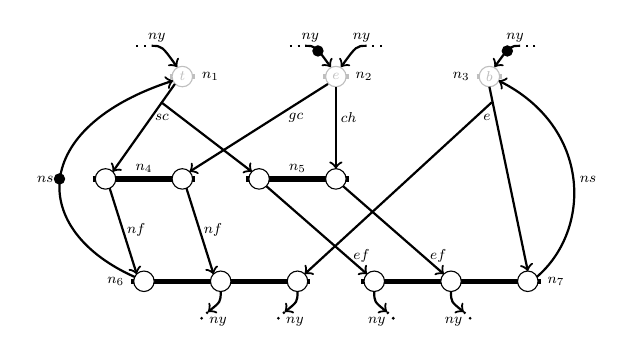
\begin{tikzpicture}[scale=0.65, every node/.style={transform shape}]

\begin{scope}[line width=2pt]
\draw (-1.75,-2) -- (0.25,-2);
\draw (1.25,-2) -- (3.25,-2);
\draw (-1,-4) -- (2.5,-4);
\draw (3.5,-4) -- (7,-4);
\end{scope}

\begin{scope}[line width=2pt, lightgray]
\draw (-0.25,0) -- (0.25,0);
\draw (2.75,0) -- (3.25,0);
\draw (5.75,0) -- (6.25,0);
\end{scope}

\filldraw [lightgray, fill=white]  (0,0)  circle (2mm) node (t0) {\footnotesize $t$};
\filldraw [lightgray, fill=white]  (3,0)  circle (2mm) node (e0) {\footnotesize $e$};
\filldraw [lightgray, fill=white]  (6,0)  circle (2mm) node (b0) {\footnotesize $b$};
\filldraw [fill=white]  (-1.5,-2)  circle (2mm) node (t1) {};
\filldraw [fill=white]  (0,-2)  circle (2mm) node (e1) {};
\filldraw [fill=white]  (1.5,-2)  circle (2mm) node (t2) {};
\filldraw [fill=white]  (3,-2)  circle (2mm) node (e2) {};
\filldraw [fill=white]  (-0.75,-4)  circle (2mm) node (t5) {};
\filldraw [fill=white]  (0.75,-4)  circle (2mm) node (e5) {};
\filldraw [fill=white]  (2.25,-4)  circle (2mm) node (b5) {};
\filldraw [fill=white]  (3.75,-4)  circle (2mm) node (t6) {};
\filldraw [fill=white]  (5.25,-4)  circle (2mm) node (e6) {};
\filldraw [fill=white]  (6.75,-4)  circle (2mm) node (b6) {};

\node at (0.55,0) {\footnotesize $n_1$};
\node at (3.55,0) {\footnotesize$n_2$};
\node at (5.45,0) {\footnotesize $n_3$};
\node at (-0.75,-1.8) {\footnotesize $n_4$};
\node at (2.25,-1.8) {\footnotesize $n_5$};
\node at (-1.3,-4) {\footnotesize $n_6$};
\node at (7.3,-4) {\footnotesize $n_7$};

\node at (-0.4, -0.8) {\footnotesize $sc$};
\node at (2.22, -0.8) {\footnotesize $gc$};
\node at (3.25, -0.8) {\footnotesize $ch$};
\node at (5.95, -0.8) {\footnotesize $e$};
\node at (-0.9,-3) {\footnotesize $nf$};
\node at (0.6, -3) {\footnotesize $nf$};
\node at (3.5,-3.5) {\footnotesize $ef$};
\node at (5,-3.5) {\footnotesize $ef$};
\node at (0.7, -4.8) {\footnotesize $ny$};
\node at (2.2, -4.8) {\footnotesize $ny$};
\node at (3.8, -4.8) {\footnotesize $ny$};
\node at (5.3, -4.8) {\footnotesize $ny$};
\node at (-0.5, 0.75) {\footnotesize $ny$};
\node at (2.5, 0.75) {\footnotesize $ny$};
\node at (3.5, 0.75) {\footnotesize $ny$};
\node at (6.5, 0.75) {\footnotesize $ny$};

\begin{scope}[thick,->]
\draw (-0.145, -0.145) -- (-1.36, -1.86); %t0-t1
\draw (-0.415, -0.5) -- (1.36, -1.86); %t0-t2
\draw (2.845, -0.145) -- (0.14, -1.86); %e0-e1
\draw (3, -0.2) -- (3, -1.8); %e0-e2
\draw (-1.5, -2) + (0.08, -0.18) -- (-0.89, -3.86); %t1-t3
\draw (0, -2) + (0.08, -0.18) -- (0.61, -3.86); %e1-e3
\draw (1.5, -2) + (0.145, -0.145) -- (3.61, -3.86); %t2-t4
\draw (3, -2) + (0.145, -0.145) -- (5.11, -3.86); %e2-e4
\draw (6.05, -0.5) -- (2.39, -3.86); %b0-b3
\draw (6, -0.2) -- (6.75, -3.8); %b0-b4
\draw (-0.92, -3.92) .. controls (-3, -3) and (-3, -1) .. (-0.18, -0.08) node [midway, left] {\footnotesize $ns$}; %t3-t0
\draw (6.92, -3.92) .. controls (8, -3) and (8, -1) .. (6.18, -0.08) node [midway, right] {\footnotesize $ns$}; %b4-b0
\draw (0.75,-4.2) .. controls (0.75, -4.4) .. (0.5,-4.6) ; %e3-e0
\draw (2.25, -4.2) .. controls (2.25, -4.4) .. (2, -4.6); %b3-b0
\draw (3.75, -4.2) .. controls (3.75, -4.4) .. (4, -4.6); %t4-t0
\draw (5.25, -4.2) .. controls (5.25, -4.4) .. (5.5, -4.6); %e4-e0
\draw (-0.6, 0.6) .. controls (-0.4, 0.6) .. (-0.1, 0.185); %t4-t0
\draw (2.4, 0.6) .. controls (2.6, 0.6) .. (2.9, 0.185); %e3-e0
\draw (3.6, 0.6) .. controls (3.4, 0.6) .. (3.1, 0.185); %e4-e0
\draw (6.6, 0.6) .. controls (6.4, 0.6) .. (6.1, 0.185); %b3-b0
\end{scope}

\begin{scope}[thick, dotted]
\draw (-0.9, 0.6) -- (-0.6, 0.6);
\draw (2.1, 0.6) -- (2.4, 0.6);
\draw (3.9, 0.6) -- (3.6, 0.6);
\draw (6.9, 0.6) -- (6.6, 0.6);
\draw (0.5,-4.6) -- (0.3, -4.8);
\draw (2, -4.6) -- (1.8, -4.8);
\draw (4, -4.6) -- (4.2, -4.8);
\draw (5.5, -4.6) -- (5.7, -4.8);
\end{scope}

\filldraw [fill=black]  (-2.4,-2)  circle (1mm);
\filldraw [fill=black]  (2.65,0.5)  circle (1mm);
\filldraw [fill=black]  (6.35,0.5)  circle (1mm);

\end{tikzpicture}
\end{minipage}
\begin{minipage}{.49\textwidth}
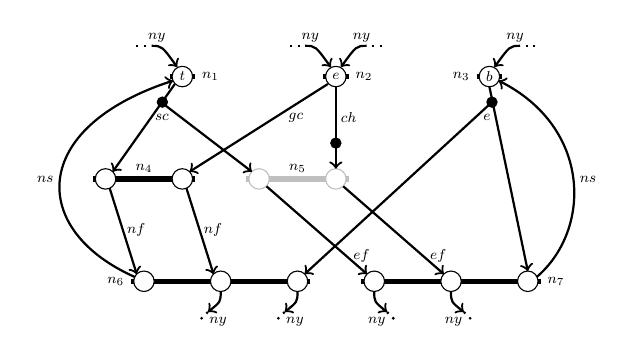
\begin{tikzpicture}[scale=0.65, every node/.style={transform shape}]

\begin{scope}[line width=2pt]
\draw (-0.25,0) -- (0.25,0);
\draw (2.75,0) -- (3.25,0);
\draw (5.75,0) -- (6.25,0);
\draw (-1.75,-2) -- (0.25,-2);
\draw (-1,-4) -- (2.5,-4);
\draw (3.5,-4) -- (7,-4);
\end{scope}

\draw [line width=2pt, lightgray] (1.25,-2) -- (3.25,-2);

\filldraw [fill=white]  (0,0)  circle (2mm) node (t0) {\footnotesize $t$};
\filldraw [fill=white]  (3,0)  circle (2mm) node (e0) {\footnotesize $e$};
\filldraw [fill=white]  (6,0)  circle (2mm) node (b0) {\footnotesize $b$};
\filldraw [fill=white]  (-1.5,-2)  circle (2mm) node (t1) {};
\filldraw [fill=white]  (0,-2)  circle (2mm) node (e1) {};
\filldraw [lightgray, fill=white]  (1.5,-2)  circle (2mm) node (t2) {};
\filldraw [lightgray, fill=white]  (3,-2)  circle (2mm) node (e2) {};
\filldraw [fill=white]  (-0.75,-4)  circle (2mm) node (t5) {};
\filldraw [fill=white]  (0.75,-4)  circle (2mm) node (e5) {};
\filldraw [fill=white]  (2.25,-4)  circle (2mm) node (b5) {};
\filldraw [fill=white]  (3.75,-4)  circle (2mm) node (t6) {};
\filldraw [fill=white]  (5.25,-4)  circle (2mm) node (e6) {};
\filldraw [fill=white]  (6.75,-4)  circle (2mm) node (b6) {};

\node at (0.55,0) {\footnotesize $n_1$};
\node at (3.55,0) {\footnotesize$n_2$};
\node at (5.45,0) {\footnotesize $n_3$};
\node at (-0.75,-1.8) {\footnotesize $n_4$};
\node at (2.25,-1.8) {\footnotesize $n_5$};
\node at (-1.3,-4) {\footnotesize $n_6$};
\node at (7.3,-4) {\footnotesize $n_7$};

\node at (-0.4, -0.8) {\footnotesize $sc$};
\node at (2.22, -0.8) {\footnotesize $gc$};
\node at (3.25, -0.8) {\footnotesize $ch$};
\node at (5.95, -0.8) {\footnotesize $e$};
\node at (-0.9,-3) {\footnotesize $nf$};
\node at (0.6, -3) {\footnotesize $nf$};
\node at (3.5,-3.5) {\footnotesize $ef$};
\node at (5,-3.5) {\footnotesize $ef$};
\node at (0.7, -4.8) {\footnotesize $ny$};
\node at (2.2, -4.8) {\footnotesize $ny$};
\node at (3.8, -4.8) {\footnotesize $ny$};
\node at (5.3, -4.8) {\footnotesize $ny$};
\node at (-0.5, 0.75) {\footnotesize $ny$};
\node at (2.5, 0.75) {\footnotesize $ny$};
\node at (3.5, 0.75) {\footnotesize $ny$};
\node at (6.5, 0.75) {\footnotesize $ny$};

\begin{scope}[thick,->]
\draw (-0.145, -0.145) -- (-1.36, -1.86); %t0-t1
\draw (-0.415, -0.5) -- (1.36, -1.86); %t0-t2
\draw (2.845, -0.145) -- (0.14, -1.86); %e0-e1
\draw (3, -0.2) -- (3, -1.8); %e0-e2
\draw (-1.5, -2) + (0.08, -0.18) -- (-0.89, -3.86); %t1-t3
\draw (0, -2) + (0.08, -0.18) -- (0.61, -3.86); %e1-e3
\draw (1.5, -2) + (0.145, -0.145) -- (3.61, -3.86); %t2-t4
\draw (3, -2) + (0.145, -0.145) -- (5.11, -3.86); %e2-e4
\draw (6.05, -0.5) -- (2.39, -3.86); %b0-b3
\draw (6, -0.2) -- (6.75, -3.8); %b0-b4
\draw (-0.92, -3.92) .. controls (-3, -3) and (-3, -1) .. (-0.18, -0.08) node [midway, left] {\footnotesize $ns$}; %t3-t0
\draw (6.92, -3.92) .. controls (8, -3) and (8, -1) .. (6.18, -0.08) node [midway, right] {\footnotesize $ns$}; %b4-b0
\draw (0.75,-4.2) .. controls (0.75, -4.4) .. (0.5,-4.6) ; %e3-e0
\draw (2.25, -4.2) .. controls (2.25, -4.4) .. (2, -4.6); %b3-b0
\draw (3.75, -4.2) .. controls (3.75, -4.4) .. (4, -4.6); %t4-t0
\draw (5.25, -4.2) .. controls (5.25, -4.4) .. (5.5, -4.6); %e4-e0
\draw (-0.6, 0.6) .. controls (-0.4, 0.6) .. (-0.1, 0.185); %t4-t0
\draw (2.4, 0.6) .. controls (2.6, 0.6) .. (2.9, 0.185); %e3-e0
\draw (3.6, 0.6) .. controls (3.4, 0.6) .. (3.1, 0.185); %e4-e0
\draw (6.6, 0.6) .. controls (6.4, 0.6) .. (6.1, 0.185); %b3-b0
\end{scope}

\begin{scope}[thick, dotted]
\draw (-0.9, 0.6) -- (-0.6, 0.6);
\draw (2.1, 0.6) -- (2.4, 0.6);
\draw (3.9, 0.6) -- (3.6, 0.6);
\draw (6.9, 0.6) -- (6.6, 0.6);
\draw (0.5,-4.6) -- (0.3, -4.8);
\draw (2, -4.6) -- (1.8, -4.8);
\draw (4, -4.6) -- (4.2, -4.8);
\draw (5.5, -4.6) -- (5.7, -4.8);
\end{scope}

\filldraw [fill=black]  (-0.39,-0.5)  circle (1mm);
\filldraw [fill=black]  (3,-1.3)  circle (1mm);
\filldraw [fill=black]  (6.05,-0.5)  circle (1mm);

\end{tikzpicture}
\end{minipage}
\begin{minipage}{.49\textwidth}
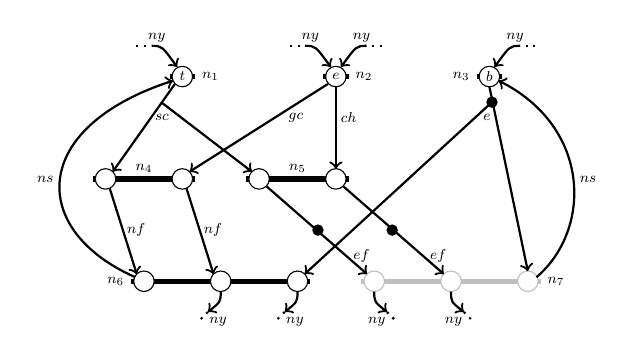
\begin{tikzpicture}[scale=0.65, every node/.style={transform shape}]

\begin{scope}[line width=2pt]
\draw (-0.25,0) -- (0.25,0);
\draw (2.75,0) -- (3.25,0);
\draw (5.75,0) -- (6.25,0);
\draw (-1.75,-2) -- (0.25,-2);
\draw (1.25,-2) -- (3.25,-2);
\draw (-1,-4) -- (2.5,-4);
\end{scope}

\draw [line width=2pt, lightgray] (3.5,-4) -- (7,-4);

\filldraw [fill=white]  (0,0)  circle (2mm) node (t0) {\footnotesize $t$};
\filldraw [fill=white]  (3,0)  circle (2mm) node (e0) {\footnotesize $e$};
\filldraw [fill=white]  (6,0)  circle (2mm) node (b0) {\footnotesize $b$};
\filldraw [fill=white]  (-1.5,-2)  circle (2mm) node (t1) {};
\filldraw [fill=white]  (0,-2)  circle (2mm) node (e1) {};
\filldraw [fill=white]  (1.5,-2)  circle (2mm) node (t2) {};
\filldraw [fill=white]  (3,-2)  circle (2mm) node (e2) {};
\filldraw [fill=white]  (-0.75,-4)  circle (2mm) node (t5) {};
\filldraw [fill=white]  (0.75,-4)  circle (2mm) node (e5) {};
\filldraw [fill=white]  (2.25,-4)  circle (2mm) node (b5) {};
\filldraw [lightgray, fill=white]  (3.75,-4)  circle (2mm) node (t6) {};
\filldraw [lightgray, fill=white]  (5.25,-4)  circle (2mm) node (e6) {};
\filldraw [lightgray, fill=white]  (6.75,-4)  circle (2mm) node (b6) {};

\node at (0.55,0) {\footnotesize $n_1$};
\node at (3.55,0) {\footnotesize$n_2$};
\node at (5.45,0) {\footnotesize $n_3$};
\node at (-0.75,-1.8) {\footnotesize $n_4$};
\node at (2.25,-1.8) {\footnotesize $n_5$};
\node at (-1.3,-4) {\footnotesize $n_6$};
\node at (7.3,-4) {\footnotesize $n_7$};

\node at (-0.4, -0.8) {\footnotesize $sc$};
\node at (2.22, -0.8) {\footnotesize $gc$};
\node at (3.25, -0.8) {\footnotesize $ch$};
\node at (5.95, -0.8) {\footnotesize $e$};
\node at (-0.9,-3) {\footnotesize $nf$};
\node at (0.6, -3) {\footnotesize $nf$};
\node at (3.5,-3.5) {\footnotesize $ef$};
\node at (5,-3.5) {\footnotesize $ef$};
\node at (0.7, -4.8) {\footnotesize $ny$};
\node at (2.2, -4.8) {\footnotesize $ny$};
\node at (3.8, -4.8) {\footnotesize $ny$};
\node at (5.3, -4.8) {\footnotesize $ny$};
\node at (-0.5, 0.75) {\footnotesize $ny$};
\node at (2.5, 0.75) {\footnotesize $ny$};
\node at (3.5, 0.75) {\footnotesize $ny$};
\node at (6.5, 0.75) {\footnotesize $ny$};

\begin{scope}[thick,->]
\draw (-0.145, -0.145) -- (-1.36, -1.86); %t0-t1
\draw (-0.415, -0.5) -- (1.36, -1.86); %t0-t2
\draw (2.845, -0.145) -- (0.14, -1.86); %e0-e1
\draw (3, -0.2) -- (3, -1.8); %e0-e2
\draw (-1.5, -2) + (0.08, -0.18) -- (-0.89, -3.86); %t1-t3
\draw (0, -2) + (0.08, -0.18) -- (0.61, -3.86); %e1-e3
\draw (1.5, -2) + (0.145, -0.145) -- (3.61, -3.86); %t2-t4
\draw (3, -2) + (0.145, -0.145) -- (5.11, -3.86); %e2-e4
\draw (6.05, -0.5) -- (2.39, -3.86); %b0-b3
\draw (6, -0.2) -- (6.75, -3.8); %b0-b4
\draw (-0.92, -3.92) .. controls (-3, -3) and (-3, -1) .. (-0.18, -0.08) node [midway, left] {\footnotesize $ns$}; %t3-t0
\draw (6.92, -3.92) .. controls (8, -3) and (8, -1) .. (6.18, -0.08) node [midway, right] {\footnotesize $ns$}; %b4-b0
\draw (0.75,-4.2) .. controls (0.75, -4.4) .. (0.5,-4.6) ; %e3-e0
\draw (2.25, -4.2) .. controls (2.25, -4.4) .. (2, -4.6); %b3-b0
\draw (3.75, -4.2) .. controls (3.75, -4.4) .. (4, -4.6); %t4-t0
\draw (5.25, -4.2) .. controls (5.25, -4.4) .. (5.5, -4.6); %e4-e0
\draw (-0.6, 0.6) .. controls (-0.4, 0.6) .. (-0.1, 0.185); %t4-t0
\draw (2.4, 0.6) .. controls (2.6, 0.6) .. (2.9, 0.185); %e3-e0
\draw (3.6, 0.6) .. controls (3.4, 0.6) .. (3.1, 0.185); %e4-e0
\draw (6.6, 0.6) .. controls (6.4, 0.6) .. (6.1, 0.185); %b3-b0
\end{scope}

\begin{scope}[thick, dotted]
\draw (-0.9, 0.6) -- (-0.6, 0.6);
\draw (2.1, 0.6) -- (2.4, 0.6);
\draw (3.9, 0.6) -- (3.6, 0.6);
\draw (6.9, 0.6) -- (6.6, 0.6);
\draw (0.5,-4.6) -- (0.3, -4.8);
\draw (2, -4.6) -- (1.8, -4.8);
\draw (4, -4.6) -- (4.2, -4.8);
\draw (5.5, -4.6) -- (5.7, -4.8);
\end{scope}

\filldraw [fill=black]  (2.65,-3)  circle (1mm);
\filldraw [fill=black]  (4.1,-3)  circle (1mm);
\filldraw [fill=black]  (6.05,-0.5)  circle (1mm);

\end{tikzpicture}
\end{minipage}
\begin{minipage}{.49\textwidth}
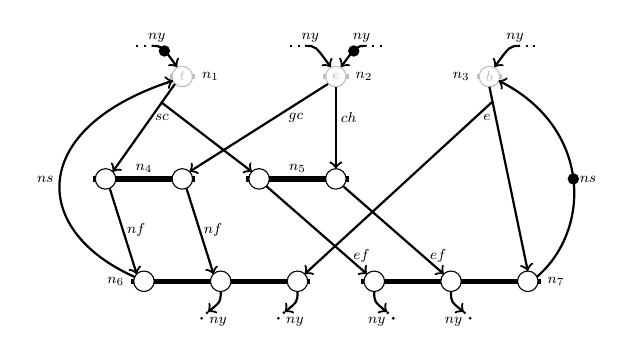
\begin{tikzpicture}[scale=0.65, every node/.style={transform shape}]

\begin{scope}[line width=2pt]
\draw (-1.75,-2) -- (0.25,-2);
\draw (1.25,-2) -- (3.25,-2);
\draw (-1,-4) -- (2.5,-4);
\draw (3.5,-4) -- (7,-4);
\end{scope}

\begin{scope}[line width=2pt, lightgray]
\draw (-0.25,0) -- (0.25,0);
\draw (2.75,0) -- (3.25,0);
\draw (5.75,0) -- (6.25,0);
\end{scope}

\filldraw [lightgray, fill=white]  (0,0)  circle (2mm) node (t0) {\footnotesize $t$};
\filldraw [lightgray, fill=white]  (3,0)  circle (2mm) node (e0) {\footnotesize $e$};
\filldraw [lightgray, fill=white]  (6,0)  circle (2mm) node (b0) {\footnotesize $b$};
\filldraw [fill=white]  (-1.5,-2)  circle (2mm) node (t1) {};
\filldraw [fill=white]  (0,-2)  circle (2mm) node (e1) {};
\filldraw [fill=white]  (1.5,-2)  circle (2mm) node (t2) {};
\filldraw [fill=white]  (3,-2)  circle (2mm) node (e2) {};
\filldraw [fill=white]  (-0.75,-4)  circle (2mm) node (t5) {};
\filldraw [fill=white]  (0.75,-4)  circle (2mm) node (e5) {};
\filldraw [fill=white]  (2.25,-4)  circle (2mm) node (b5) {};
\filldraw [fill=white]  (3.75,-4)  circle (2mm) node (t6) {};
\filldraw [fill=white]  (5.25,-4)  circle (2mm) node (e6) {};
\filldraw [fill=white]  (6.75,-4)  circle (2mm) node (b6) {};

\node at (0.55,0) {\footnotesize $n_1$};
\node at (3.55,0) {\footnotesize$n_2$};
\node at (5.45,0) {\footnotesize $n_3$};
\node at (-0.75,-1.8) {\footnotesize $n_4$};
\node at (2.25,-1.8) {\footnotesize $n_5$};
\node at (-1.3,-4) {\footnotesize $n_6$};
\node at (7.3,-4) {\footnotesize $n_7$};

\node at (-0.4, -0.8) {\footnotesize $sc$};
\node at (2.22, -0.8) {\footnotesize $gc$};
\node at (3.25, -0.8) {\footnotesize $ch$};
\node at (5.95, -0.8) {\footnotesize $e$};
\node at (-0.9,-3) {\footnotesize $nf$};
\node at (0.6, -3) {\footnotesize $nf$};
\node at (3.5,-3.5) {\footnotesize $ef$};
\node at (5,-3.5) {\footnotesize $ef$};
\node at (0.7, -4.8) {\footnotesize $ny$};
\node at (2.2, -4.8) {\footnotesize $ny$};
\node at (3.8, -4.8) {\footnotesize $ny$};
\node at (5.3, -4.8) {\footnotesize $ny$};
\node at (-0.5, 0.75) {\footnotesize $ny$};
\node at (2.5, 0.75) {\footnotesize $ny$};
\node at (3.5, 0.75) {\footnotesize $ny$};
\node at (6.5, 0.75) {\footnotesize $ny$};

\begin{scope}[thick,->]
\draw (-0.145, -0.145) -- (-1.36, -1.86); %t0-t1
\draw (-0.415, -0.5) -- (1.36, -1.86); %t0-t2
\draw (2.845, -0.145) -- (0.14, -1.86); %e0-e1
\draw (3, -0.2) -- (3, -1.8); %e0-e2
\draw (-1.5, -2) + (0.08, -0.18) -- (-0.89, -3.86); %t1-t3
\draw (0, -2) + (0.08, -0.18) -- (0.61, -3.86); %e1-e3
\draw (1.5, -2) + (0.145, -0.145) -- (3.61, -3.86); %t2-t4
\draw (3, -2) + (0.145, -0.145) -- (5.11, -3.86); %e2-e4
\draw (6.05, -0.5) -- (2.39, -3.86); %b0-b3
\draw (6, -0.2) -- (6.75, -3.8); %b0-b4
\draw (-0.92, -3.92) .. controls (-3, -3) and (-3, -1) .. (-0.18, -0.08) node [midway, left] {\footnotesize $ns$}; %t3-t0
\draw (6.92, -3.92) .. controls (8, -3) and (8, -1) .. (6.18, -0.08) node [midway, right] {\footnotesize $ns$}; %b4-b0
\draw (0.75,-4.2) .. controls (0.75, -4.4) .. (0.5,-4.6) ; %e3-e0
\draw (2.25, -4.2) .. controls (2.25, -4.4) .. (2, -4.6); %b3-b0
\draw (3.75, -4.2) .. controls (3.75, -4.4) .. (4, -4.6); %t4-t0
\draw (5.25, -4.2) .. controls (5.25, -4.4) .. (5.5, -4.6); %e4-e0
\draw (-0.6, 0.6) .. controls (-0.4, 0.6) .. (-0.1, 0.185); %t4-t0
\draw (2.4, 0.6) .. controls (2.6, 0.6) .. (2.9, 0.185); %e3-e0
\draw (3.6, 0.6) .. controls (3.4, 0.6) .. (3.1, 0.185); %e4-e0
\draw (6.6, 0.6) .. controls (6.4, 0.6) .. (6.1, 0.185); %b3-b0
\end{scope}

\begin{scope}[thick, dotted]
\draw (-0.9, 0.6) -- (-0.6, 0.6);
\draw (2.1, 0.6) -- (2.4, 0.6);
\draw (3.9, 0.6) -- (3.6, 0.6);
\draw (6.9, 0.6) -- (6.6, 0.6);
\draw (0.5,-4.6) -- (0.3, -4.8);
\draw (2, -4.6) -- (1.8, -4.8);
\draw (4, -4.6) -- (4.2, -4.8);
\draw (5.5, -4.6) -- (5.7, -4.8);
\end{scope}

\filldraw [fill=black]  (-0.35,0.5)  circle (1mm);
\filldraw [fill=black]  (3.35,0.5)  circle (1mm);
\filldraw [fill=black]  (7.64,-2)  circle (1mm);

\end{tikzpicture}
\end{minipage}
\begin{minipage}{.49\textwidth}
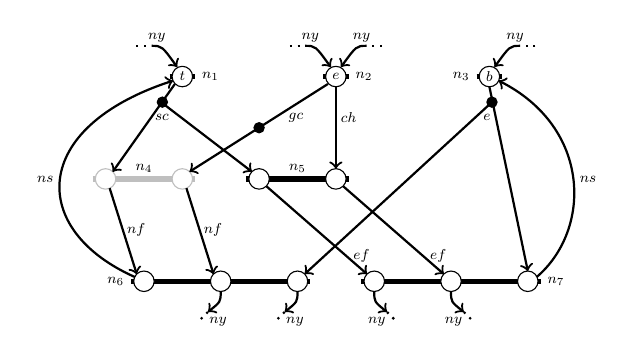
\begin{tikzpicture}[scale=0.65, every node/.style={transform shape}]

\begin{scope}[line width=2pt]
\draw (-0.25,0) -- (0.25,0);
\draw (2.75,0) -- (3.25,0);
\draw (5.75,0) -- (6.25,0);
\draw (1.25,-2) -- (3.25,-2);
\draw (-1,-4) -- (2.5,-4);
\draw (3.5,-4) -- (7,-4);
\end{scope}

\draw [line width=2pt, lightgray] (-1.75,-2) -- (0.25,-2);

\filldraw [fill=white]  (0,0)  circle (2mm) node (t0) {\footnotesize $t$};
\filldraw [fill=white]  (3,0)  circle (2mm) node (e0) {\footnotesize $e$};
\filldraw [fill=white]  (6,0)  circle (2mm) node (b0) {\footnotesize $b$};
\filldraw [lightgray, fill=white]  (-1.5,-2)  circle (2mm) node (t1) {};
\filldraw [lightgray, fill=white]  (0,-2)  circle (2mm) node (e1) {};
\filldraw [fill=white]  (1.5,-2)  circle (2mm) node (t2) {};
\filldraw [fill=white]  (3,-2)  circle (2mm) node (e2) {};
\filldraw [fill=white]  (-0.75,-4)  circle (2mm) node (t5) {};
\filldraw [fill=white]  (0.75,-4)  circle (2mm) node (e5) {};
\filldraw [fill=white]  (2.25,-4)  circle (2mm) node (b5) {};
\filldraw [fill=white]  (3.75,-4)  circle (2mm) node (t6) {};
\filldraw [fill=white]  (5.25,-4)  circle (2mm) node (e6) {};
\filldraw [fill=white]  (6.75,-4)  circle (2mm) node (b6) {};

\node at (0.55,0) {\footnotesize $n_1$};
\node at (3.55,0) {\footnotesize$n_2$};
\node at (5.45,0) {\footnotesize $n_3$};
\node at (-0.75,-1.8) {\footnotesize $n_4$};
\node at (2.25,-1.8) {\footnotesize $n_5$};
\node at (-1.3,-4) {\footnotesize $n_6$};
\node at (7.3,-4) {\footnotesize $n_7$};

\node at (-0.4, -0.8) {\footnotesize $sc$};
\node at (2.22, -0.8) {\footnotesize $gc$};
\node at (3.25, -0.8) {\footnotesize $ch$};
\node at (5.95, -0.8) {\footnotesize $e$};
\node at (-0.9,-3) {\footnotesize $nf$};
\node at (0.6, -3) {\footnotesize $nf$};
\node at (3.5,-3.5) {\footnotesize $ef$};
\node at (5,-3.5) {\footnotesize $ef$};
\node at (0.7, -4.8) {\footnotesize $ny$};
\node at (2.2, -4.8) {\footnotesize $ny$};
\node at (3.8, -4.8) {\footnotesize $ny$};
\node at (5.3, -4.8) {\footnotesize $ny$};
\node at (-0.5, 0.75) {\footnotesize $ny$};
\node at (2.5, 0.75) {\footnotesize $ny$};
\node at (3.5, 0.75) {\footnotesize $ny$};
\node at (6.5, 0.75) {\footnotesize $ny$};

\begin{scope}[thick,->]
\draw (-0.145, -0.145) -- (-1.36, -1.86); %t0-t1
\draw (-0.415, -0.5) -- (1.36, -1.86); %t0-t2
\draw (2.845, -0.145) -- (0.14, -1.86); %e0-e1
\draw (3, -0.2) -- (3, -1.8); %e0-e2
\draw (-1.5, -2) + (0.08, -0.18) -- (-0.89, -3.86); %t1-t3
\draw (0, -2) + (0.08, -0.18) -- (0.61, -3.86); %e1-e3
\draw (1.5, -2) + (0.145, -0.145) -- (3.61, -3.86); %t2-t4
\draw (3, -2) + (0.145, -0.145) -- (5.11, -3.86); %e2-e4
\draw (6.05, -0.5) -- (2.39, -3.86); %b0-b3
\draw (6, -0.2) -- (6.75, -3.8); %b0-b4
\draw (-0.92, -3.92) .. controls (-3, -3) and (-3, -1) .. (-0.18, -0.08) node [midway, left] {\footnotesize $ns$}; %t3-t0
\draw (6.92, -3.92) .. controls (8, -3) and (8, -1) .. (6.18, -0.08) node [midway, right] {\footnotesize $ns$}; %b4-b0
\draw (0.75,-4.2) .. controls (0.75, -4.4) .. (0.5,-4.6) ; %e3-e0
\draw (2.25, -4.2) .. controls (2.25, -4.4) .. (2, -4.6); %b3-b0
\draw (3.75, -4.2) .. controls (3.75, -4.4) .. (4, -4.6); %t4-t0
\draw (5.25, -4.2) .. controls (5.25, -4.4) .. (5.5, -4.6); %e4-e0
\draw (-0.6, 0.6) .. controls (-0.4, 0.6) .. (-0.1, 0.185); %t4-t0
\draw (2.4, 0.6) .. controls (2.6, 0.6) .. (2.9, 0.185); %e3-e0
\draw (3.6, 0.6) .. controls (3.4, 0.6) .. (3.1, 0.185); %e4-e0
\draw (6.6, 0.6) .. controls (6.4, 0.6) .. (6.1, 0.185); %b3-b0
\end{scope}

\begin{scope}[thick, dotted]
\draw (-0.9, 0.6) -- (-0.6, 0.6);
\draw (2.1, 0.6) -- (2.4, 0.6);
\draw (3.9, 0.6) -- (3.6, 0.6);
\draw (6.9, 0.6) -- (6.6, 0.6);
\draw (0.5,-4.6) -- (0.3, -4.8);
\draw (2, -4.6) -- (1.8, -4.8);
\draw (4, -4.6) -- (4.2, -4.8);
\draw (5.5, -4.6) -- (5.7, -4.8);
\end{scope}

\filldraw [fill=black]  (-0.39,-0.5)  circle (1mm);
\filldraw [fill=black]  (1.5,-1)  circle (1mm);
\filldraw [fill=black]  (6.05,-0.5)  circle (1mm);

\end{tikzpicture}
\end{minipage}
\begin{minipage}{.49\textwidth}
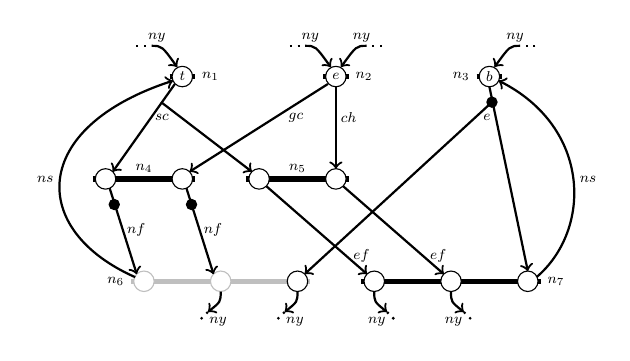
\begin{tikzpicture}[scale=0.65, every node/.style={transform shape}]

\begin{scope}[line width=2pt]
\draw (-0.25,0) -- (0.25,0);
\draw (2.75,0) -- (3.25,0);
\draw (5.75,0) -- (6.25,0);
\draw (-1.75,-2) -- (0.25,-2);
\draw (1.25,-2) -- (3.25,-2);
\draw (3.5,-4) -- (7,-4);
\end{scope}

\draw [line width=2pt, lightgray] (-1,-4) -- (2.5,-4);

\filldraw [fill=white]  (0,0)  circle (2mm) node (t0) {\footnotesize $t$};
\filldraw [fill=white]  (3,0)  circle (2mm) node (e0) {\footnotesize $e$};
\filldraw [fill=white]  (6,0)  circle (2mm) node (b0) {\footnotesize $b$};
\filldraw [fill=white]  (-1.5,-2)  circle (2mm) node (t1) {};
\filldraw [fill=white]  (0,-2)  circle (2mm) node (e1) {};
\filldraw [fill=white]  (1.5,-2)  circle (2mm) node (t2) {};
\filldraw [fill=white]  (3,-2)  circle (2mm) node (e2) {};
\filldraw [lightgray, fill=white]  (-0.75,-4)  circle (2mm) node (t5) {};
\filldraw [lightgray, fill=white]  (0.75,-4)  circle (2mm) node (e5) {};
\filldraw [fill=white]  (2.25,-4)  circle (2mm) node (b5) {};
\filldraw [fill=white]  (3.75,-4)  circle (2mm) node (t6) {};
\filldraw [fill=white]  (5.25,-4)  circle (2mm) node (e6) {};
\filldraw [fill=white]  (6.75,-4)  circle (2mm) node (b6) {};

\node at (0.55,0) {\footnotesize $n_1$};
\node at (3.55,0) {\footnotesize$n_2$};
\node at (5.45,0) {\footnotesize $n_3$};
\node at (-0.75,-1.8) {\footnotesize $n_4$};
\node at (2.25,-1.8) {\footnotesize $n_5$};
\node at (-1.3,-4) {\footnotesize $n_6$};
\node at (7.3,-4) {\footnotesize $n_7$};

\node at (-0.4, -0.8) {\footnotesize $sc$};
\node at (2.22, -0.8) {\footnotesize $gc$};
\node at (3.25, -0.8) {\footnotesize $ch$};
\node at (5.95, -0.8) {\footnotesize $e$};
\node at (-0.9,-3) {\footnotesize $nf$};
\node at (0.6, -3) {\footnotesize $nf$};
\node at (3.5,-3.5) {\footnotesize $ef$};
\node at (5,-3.5) {\footnotesize $ef$};
\node at (0.7, -4.8) {\footnotesize $ny$};
\node at (2.2, -4.8) {\footnotesize $ny$};
\node at (3.8, -4.8) {\footnotesize $ny$};
\node at (5.3, -4.8) {\footnotesize $ny$};
\node at (-0.5, 0.75) {\footnotesize $ny$};
\node at (2.5, 0.75) {\footnotesize $ny$};
\node at (3.5, 0.75) {\footnotesize $ny$};
\node at (6.5, 0.75) {\footnotesize $ny$};

\begin{scope}[thick,->]
\draw (-0.145, -0.145) -- (-1.36, -1.86); %t0-t1
\draw (-0.415, -0.5) -- (1.36, -1.86); %t0-t2
\draw (2.845, -0.145) -- (0.14, -1.86); %e0-e1
\draw (3, -0.2) -- (3, -1.8); %e0-e2
\draw (-1.5, -2) + (0.08, -0.18) -- (-0.89, -3.86); %t1-t3
\draw (0, -2) + (0.08, -0.18) -- (0.61, -3.86); %e1-e3
\draw (1.5, -2) + (0.145, -0.145) -- (3.61, -3.86); %t2-t4
\draw (3, -2) + (0.145, -0.145) -- (5.11, -3.86); %e2-e4
\draw (6.05, -0.5) -- (2.39, -3.86); %b0-b3
\draw (6, -0.2) -- (6.75, -3.8); %b0-b4
\draw (-0.92, -3.92) .. controls (-3, -3) and (-3, -1) .. (-0.18, -0.08) node [midway, left] {\footnotesize $ns$}; %t3-t0
\draw (6.92, -3.92) .. controls (8, -3) and (8, -1) .. (6.18, -0.08) node [midway, right] {\footnotesize $ns$}; %b4-b0
\draw (0.75,-4.2) .. controls (0.75, -4.4) .. (0.5,-4.6) ; %e3-e0
\draw (2.25, -4.2) .. controls (2.25, -4.4) .. (2, -4.6); %b3-b0
\draw (3.75, -4.2) .. controls (3.75, -4.4) .. (4, -4.6); %t4-t0
\draw (5.25, -4.2) .. controls (5.25, -4.4) .. (5.5, -4.6); %e4-e0
\draw (-0.6, 0.6) .. controls (-0.4, 0.6) .. (-0.1, 0.185); %t4-t0
\draw (2.4, 0.6) .. controls (2.6, 0.6) .. (2.9, 0.185); %e3-e0
\draw (3.6, 0.6) .. controls (3.4, 0.6) .. (3.1, 0.185); %e4-e0
\draw (6.6, 0.6) .. controls (6.4, 0.6) .. (6.1, 0.185); %b3-b0
\end{scope}

\begin{scope}[thick, dotted]
\draw (-0.9, 0.6) -- (-0.6, 0.6);
\draw (2.1, 0.6) -- (2.4, 0.6);
\draw (3.9, 0.6) -- (3.6, 0.6);
\draw (6.9, 0.6) -- (6.6, 0.6);
\draw (0.5,-4.6) -- (0.3, -4.8);
\draw (2, -4.6) -- (1.8, -4.8);
\draw (4, -4.6) -- (4.2, -4.8);
\draw (5.5, -4.6) -- (5.7, -4.8);
\end{scope}

\filldraw [fill=black]  (-1.33,-2.5)  circle (1mm);
\filldraw [fill=black]  (0.18,-2.5)  circle (1mm);
\filldraw [fill=black]  (6.05,-0.5)  circle (1mm);

\end{tikzpicture}
\end{minipage}
\caption{A possible run of the negotiation in Figure~\ref{fig:pollination}. Tokens represent the current readiness of each process. Gray nodes denote enabled nodes. The run illustrates how choices at \(n_1\), \(n_2\), and \(n_3\) propagate to subsequent flowering and synchronization behaviour.}
\label{fig:run}
\end{figure}

\subsection{Relation to Standard Negotiations with Transformers}
\label{sec:standard-def}

The negotiation model presented in Section~\ref{sec:negotiations} abstracts away internal agent states and transformers. For completeness and to connect with the original literature~\cite{EsparzaDeselNegotiations}, we briefly recall the standard definition and establish equivalence for control-flow properties. For the purposes of this thesis, the internal state evolution carried by transformers plays no role in enabling or disabling interactions.

\paragraph{Standard definition (informal).} In the original model, each agent $p$ has an internal state space $Q_p$ with initial states $Q_{0p}$. An atom $n$ involves parties $P_n$ and has outcomes $R_n$. Each outcome $r$ is associated with a \emph{transformer} $\tau_r$: a left-total relation $\tau_r \subseteq Q_A \times Q_A$ (where $Q_A = \prod_{p \in P} Q_p$) that is a $P_n$-transformer—it only affects states of agents in $P_n$.

When outcome $(n,r)$ occurs, agents in $P_n$ change states according to $\tau_r$, while agents outside $P_n$ remain unchanged. Crucially, \emph{enablement of an atom depends only on readiness}, not on the specific internal states of agents. The choice of outcome is non-deterministic and not restricted by internal states. Transformers determine only how internal states evolve \emph{after} an outcome occurs.

\paragraph{Why the simplification suffices.} Since this thesis focuses on reachability and control-flow properties, internal states are orthogonal: they do not influence which atoms are enabled or which outcomes can occur. All information relevant to reachability is captured by tracking which nodes each agent is ready for—exactly what markings record in our simplified definition.

\paragraph{Equivalence.}
The simplified definition of negotiations used in this thesis is equivalent to the standard definition with internal states and transformers, as far as reachability is concerned. Formally, from a standard negotiation one obtains the simplified model by projecting away internal states and retaining only the next-atom relation, which fully determines enablement and control flow. This simplification is semantic rather than approximate: it preserves the reachability graph exactly. Conversely, any simplified negotiation can be viewed as a standard one by equipping each agent with a trivial one-state internal domain and identity transformers. In both cases, the induced reachability graphs coincide. In both constructions, there is a bijection between reachable markings preserving enabled atoms and outcome occurrences. Occurrence sequences and reachability graphs correspond exactly. Properties expressible in terms of control flow (e.g., reachability, deadlock) are preserved.

\subsection{Reachability and known complexity}
\label{subsec:prelim-neg-complexity}

The central decision problem for negotiations is reachability of a marking from the initial marking. This already captures safety questions, deadlock detection, and goal attainment. For unrestricted negotiations, reachability is decidable but can be computationally expensive; in particular, the size of the reachability graph can grow exponentially. Several analysis problems for negotiations are PSPACE-hard in general. For important restricted classes, including acyclic or sound fragments, the complexity may drop substantially~\cite{EsparzaDeselNegotiations,EsparzaWorkflow,EsparzaFreeChoice}.

For the purposes of this thesis, the main point is not the exact untimed complexity landscape, but the structural character of the model: negotiations provide an explicit control-flow semantics in which multiparty interaction is primitive. That is the concurrency ingredient that LTNs retain.
%add other results

\subsection{Relation to standard negotiations and to Petri nets}
\label{subsec:prelim-neg-relations}

%Two remarks place the simplified presentation of negotiations used in this thesis in a broader formal context.

%\paragraph{Relation to standard negotiations with transformers.} The original definition of negotiations~\cite{EsparzaDeselNegotiations,DeselEsparzaNegPN} equips each atomic negotiation outcome with a \emph{transformer} acting on the internal states of the participating agents. Formally, if \(A\) is the set of agents and each agent \(a\in A\) has a local state space \(Q_a\), then a transformer is a left-total relation on the product \(Q_A=\prod_{a\in A} Q_a\), and an outcome of an atom with participant set \(P\subseteq A\) carries a \(P\)-transformer, meaning that it may change only the local states of agents in \(P\).

%For the purposes of the present thesis, these internal states are not needed. They do not influence which nodes are enabled or which outcomes may occur; they only update additional data associated with agents after an outcome has been chosen. Since our later decision problems concern reachability of control configurations rather than data-dependent properties, we work with a control-flow abstraction in which the semantic state of a negotiation is given only by its marking. In this sense, the simplified model used here should be understood as the control skeleton of the standard one.

\paragraph{Relation to Petri nets.}
A more precise connection with Petri nets is developed by Desel and
Esparza~\cite{DeselEsparzaNegPN}. They show that every negotiation can be
translated into an associated \emph{1-safe labelled Petri net}. The translation
is behaviour-preserving in a strong sense: the label reachability graph of the
negotiation is isomorphic to the label reachability graph of the associated
labelled Petri net, and likewise the concurrent-step reachability graph is
preserved. Thus, both sequential behaviour and the concurrency structure of the
negotiation are faithfully reflected in the net.

The translation can be sketched as follows. For each agent \(a\) and each set of
atoms \(X\) that may be simultaneously ready for \(a\), one introduces a place
\([a,X]\), interpreted as saying that agent \(a\) is currently ready to engage in
exactly the atoms of \(X\). For each outcome \((n,r)\), one introduces a family
of Petri-net transitions labelled by \((n,r)\), one for each possible
combination of readiness places that enables the occurrence of \(n\). Such a
transition consumes one readiness token for each participating agent and
produces the new readiness tokens prescribed by the negotiation's transition
function. As a consequence of this construction, the associated net is 1-safe.

This translation also clarifies where the main structural difference lies. In the
general case, the associated Petri net may be exponentially larger than the
negotiation, because proper hyperarcs may give rise to many combinations of
input places. For \emph{deterministic} negotiations, however, the situation is
better: the associated Petri net has only linear size, it is a
\emph{free-choice} net, and soundness is preserved in the workflow-net setting
via place equivalence. Conversely, every sound free-choice workflow net is place
equivalent to a net associated with a sound deterministic negotiation. These
results explain why negotiations may be viewed as a structurally disciplined
interaction-centric subclass of workflow-style Petri-net behaviour.

For this thesis, the main consequence is conceptual. Negotiations are close
enough to Petri nets to inherit a robust concurrency-theoretic interpretation,
yet explicit enough to let us work directly with participants, outcomes, and
readiness. This is exactly the level of abstraction at which we later add local
quantitative time.

Negotiations have been applied to the analysis of business processes, often modelled by workflow Petri nets~\cite{EsparzaWorkflow}. Such nets underlie popular graphical notations like BPMN, EPC, and UML Activity Diagrams~\cite{DijkmanBPMN}. Deterministic negotiations are closely related to free-choice workflow nets~\cite{EsparzaFreeChoice}, which are expressive enough for many industrial processes; empirical studies show that a large fraction of real-world models fall into the free-choice class.

In the remainder of the thesis, we extend negotiations with quantitative timing information, in the form of local clocks and time constraints, and study reachability in this enriched model.

%________________________________________________________________________________________________
\section{Timed Automata}
\label{sec:prelim-ta}

Timed automata~\cite{AlurDillTA} extend finite automata with real-valued clock variables that evolve continuously with time. They provide the standard framework for modeling and verifying real-time systems, and form the semantic foundation for the timing aspects of local-timed negotiations.

We briefly recall their definition, operational semantics, and the region-based decidability result for reachability, which will serve as a conceptual template for later constructions. This material is standard; we include it to establish notation and to highlight which techniques transfer (or fail to transfer) to local-timed negotiations.

\subsection{Syntax and Semantics}

We work in dense time over the non-negative reals $\mathbb{R}_{\geq 0}$. All clocks evolve synchronously with global time in standard timed automata.

\paragraph{Clock constraints.} Let $X$ be a finite set of \emph{clocks}. A \emph{clock valuation} is a function $v : X \to \mathbb{R}_{\geq 0}$. For $\delta \in \mathbb{R}_{\geq 0}$, we write $v + \delta$ for the valuation $(v + \delta)(x) = v(x) + \delta$ (uniform time elapse). For $Y \subseteq X$, we write $[Y]v$ for the valuation that resets clocks in $Y$ to zero: $([Y]v)(x) = 0$ if $x \in Y$, and $([Y]v)(x) = v(x)$ otherwise.

The set of \emph{clock constraints} over $X$, denoted $\mathcal{C}(X)$, is defined by the grammar:
\[
g ::= x \bowtie c \mid g \wedge g
\]
where $x \in X$, $c \in \mathbb{N}$, and $\bowtie \in \{<, \leq, =, \geq, >\}$. A valuation $v$ \emph{satisfies} constraint $g$, written $v \models g$, if $g$ evaluates to true when each clock $x$ is replaced by $v(x)$.

\begin{definition}[Timed automaton]
\label{def:timed-automaton}
A \textsf{timed automaton} (TA) is a tuple $\mathcal{A} = (Q, \S, X, T, q_0, \text{Acc})$ where:
\begin{itemize}
\item $Q$ is a finite set of \emph{states} (or \emph{locations}),
\item $\S$ is a finite \emph{alphabet} of actions,
\item $X$ is a finite set of \emph{clocks},
\item $q_0 \in Q$ is the \emph{initial state},
\item $\text{Acc} \subseteq Q$ is the set of \emph{accepting states},
\item $T \subseteq Q \times \S \times \mathcal{C}(X) \times 2^X \times Q$ is a finite set of \emph{transitions}. A transition $(q, a, g, R, q') \in T$ has source state $q$, action label $a$, guard $g$, reset set $R$, and target state $q'$.
\end{itemize}
\end{definition}

\paragraph{Semantics.} The behavior of $\mathcal{A}$ is given by an infinite-state transition system whose \emph{configurations} are pairs $(q, v)$ consisting of a state $q \in Q$ and a valuation $v : X \to \mathbb{R}_{\geq 0}$. The \emph{initial configuration} is $(q_0, \mathbf{0})$ where $\mathbf{0}$ denotes the valuation assigning zero to all clocks.

There are two kinds of transitions:
\begin{itemize}
\item \textbf{Delay transitions:} $(q, v) \xrightarrow{\delta} (q, v + \delta)$ for any $\delta \in \mathbb{R}_{\geq 0}$. Time elapses uniformly for all clocks.
\item \textbf{Action transitions:} $(q, v) \xrightarrow{a} (q', v')$ if there exists a transition $(q, a, g, R, q') \in T$ such that $v \models g$ and $v' = [R]v$. The guard must be satisfied, and clocks in $R$ are reset.
\end{itemize}

A \emph{run} is a finite or infinite alternating sequence of delay and action transitions starting from the initial configuration:
\[
(q_0, \mathbf{0}) \xrightarrow{\delta_0} (q_0, v_0) \xrightarrow{a_0} (q_1, v_1) \xrightarrow{\delta_1} (q_1, v_1') \xrightarrow{a_1} (q_2, v_2) \xrightarrow{\delta_2} \cdots
\]
We often write $(q, v) \xrightarrow{\delta, a} (q', v')$ to denote a delay $\delta$ followed immediately by action $a$. A run is \emph{accepting} if it reaches some configuration $(q_f, v)$ with $q_f \in \text{Acc}$.

\paragraph{A small example.}
A useful mental picture is the following two-clock automaton. One clock $x$ measures how long the system has waited since the last $a$-transition, while another clock $y$ measures the total elapsed time since the start. A transition labelled $a$ may only be taken while $x \leq 2$, and taking it resets $x$. A later transition labelled $b$ becomes available only when $y \geq 10$. This tiny example already exhibits the central tension of timed automata: the system has finitely many control locations but infinitely many possible valuations.

\begin{definition}[Reachability problem for TA]
Given a timed automaton $\mathcal{A}$ and a target state $q_{\text{target}} \in Q$, the \textsf{reachability problem} asks: does there exist an accepting run reaching some configuration $(q_{\text{target}}, v)$?
\end{definition}

\subsection{Region Abstraction and Decidability~\cite{}}

For this thesis, regions serve as the main conceptual tool for proving decidability and establishing complexity bounds, in particular as a reference point when extending negotiations with local time. We therefore briefly recall the region abstraction for timed automata, focusing on the properties needed later.

Since the transition system of a timed automaton is infinite, the standard approach is to construct a finite abstraction by grouping clock valuations that are indistinguishable with respect to future behaviour. Concretely, two valuations are grouped together if they enable the same transitions and allow the same sequences of discrete states to be reached, possibly with different delays. This yields a finite partition of the valuation space into regions, and a corresponding finite region graph obtained by combining regions with control states. For reachability, the exact delays are irrelevant; only the existence of a run following a given sequence of transitions matters.

Let $X$ be a finite set of clocks. Let $M : X \xra N \cup \{-\infty\}$ be a bound function that associates a constant $M_x \in N$ to every clock $x$.

\begin{definition}[Region equivalence \cite{}]
Two valuations $v, v' \in \Rpos$ are region equivalent w.r.t. $M$, denoted $v \sim_M v'$ iff for every $x, y \in X$:
\begin{itemize}
	\item $v(x) > M_x$ iff $v'(x) > M_x$;
	\item if $v(x) \leq M_x$, then $\lceil v(x) \rceil = \lceil v'(x) \rceil$;
	\item if $v(x) \leq M_x$, then $\{v(x)\} = 0$ iff $\{v'(x)\} = 0$;
	\item if $v(x) \leq M_x$ and $v(y) \leq M_y$ then $\{v(x)\} \leq \{v(y)\}$ iff $\{v'(x)\} \leq \{v'(y)\}$.
\end{itemize}
\end{definition}

Given a timed automaton $A$, a bound function is obtained by choosing for a clock $x$, the maximum constant appearing in a guard involving $x$. Then, the first three conditions in the above definition ensure that the two valuations satisfy the same guards. The last one enforces that for every $\d \in \Rpos$ there is $\d' \in \Rpos$, such that valuations $v + \d$ and $v' + \d'$ satisfy the same guards.

\begin{definition}[Regions \cite{}]
Let $M : X \xra{} \N \cup \{-\infty\}$ be a bound function. A region is an equivalence class of $\sim_M$. We write $[v]^M$ for the region of $v$, and $\calR_M$ for the set of all regions with respect to $M$.
\end{definition}

Figure~\ref{} shows the division into regions when there are two clocks $x$ and $y$. We also give below a constructive definition of regions which would be useful to estimate the number of regions.

\begin{definition}[Region: constructive definition \cite{}]
A region with respect to bound function $M$ is a set of valuations specified as follows:
\begin{itemize}
	\item for each clock $x \in X$, one constraint from the set: $\{x = c \mid c = 0, \dots, M_x\} \cup \{c - 1 < x < c \mid c = 1, \dots, M_x\} \cup \{x > M_x\}$
	\item for each pair of clocks $x, y$ having interval constraints: $c - 1 < x < c$ and $d - 1 < y < d$, it is specified if $\{x\}$ is less than, equal to or greater than $\{y\}$.
\end{itemize}
\end{definition}

If $r$ is a region then we will write $r \models g$ to mean that every valuation in $r$ satisfies the guard $g$. It is straightforward to see that if a valuation $v \in r$ satisfies the guard $g$, then every valuation $v' \in r$ satisfies $g$. We will now show the other property with respect to time-elapse mentioned above.

\begin{lemma}
Let $v, v'$ be valuations such that $v' \sim v$. Then, for all $\d \in \Rpos$ there exists a $\d' \in \Rpos$ such that $v' + \d' \sim_M v + \d$.
\end{lemma}

\begin{proof}
Let $v' \sim v$ and fix $\d \in \Rpos$. We construct $\d'$. Put $\lceil \d' \rceil$ to be $\lceil \d \rceil$. Clearly, we have $v' + \lceil \d' \rceil \sim_M \lceil \d \rceil$: that is, valuations $v' + \lceil \d' \rceil$ and $v + \lceil \d \rceil$ have the same integral parts and the same ordering of fractional parts (modulo $M$). Let $x_1 \lessdot_1 x_2 \lessdot_2 \cdots \lessdot_{k - 1} x_k$ be the ordering of fractional parts of clocks less than $M$ in both the valuations. Here $\lessdot$ denotes either $<$ or $=$. 

From $v + \lceil \d \rceil$, elapsing a fractional amount $\{\d\}$ might move some of the clocks up to the next integer. Let $x_j, x_{j + 1}, \dots, x_k$ be the clocks that have their integral values increased from $v + \lceil \d \rceil$ due to the fractional elapse $\{\d\}$. Thanks to the denseness of the real line, one can choose $\{\d'\}$ between the fractional values of clocks $x_{j - 1}$ and $x_j$ in $v' + \lceil \d' \rceil$ so that $v' + \d'$ has the same integers as $v + \d$ and the same ordering of fractional parts (modulo $M$).
\end{proof}

Given a bound function $M$, the number of regions in $\calR_M$ is finite. Once this finite partition of the valuations is obtained, we proceed to define a finite graph built from these regions, that captures the behaviour of the timed automaton. For an automaton $A$, to define its region graph, we consider a bound function $M_A$ that is obtained from the automaton’s definition.

\begin{definition}[Maximal bounds]
Given an automaton $A$, the maximal bounds function $M_A: X \xra{} \N \cup \{-\infty\}$ associates to each clock $x$ the biggest constant appearing in a guard of the automaton that involves $x$. If there is no guard involving $x$, then $M_A(x)$ is assigned $-\infty$.
\end{definition}

We define the region graph of an automaton $A$ using the $\sim_{M_A}$ relation. Note that in class, we used the terminology region automaton. As we are not interested in the language accepted by this automaton, and instead we care if there is a path to the accepting state, we will stick to calling this a region graph.

\begin{definition}[Region graph \cite{}]
Nodes of the region graph denoted by $RG(A)$ are of the form $(q, r)$ for $q$ a state of $A$ and $r \in \calR_{M_A}$ a region. There is a transition $(q, r) \xra{t} (q', r')$ if there are $v \in r, \d \in \Rpos$ and $v' \in r'$ with $(q, v) \xra{\d, t} (q', v')$. The initial node of the region graph is $(q_0, [0]_{\sim_{M_A}})$ where $[0]_{\sim_{M_A}}$ represents the region to which the initial valuation $0$ belongs to. A node $(q, r)$ is said to be an accepting node if $q \in Acc$.
\end{definition}

A key property of region graphs is pre-stability, which ensures that transitions are representative of all valuations in a region.

\begin{lemma}[Pre-stability of regions]
\label{lem:prestability}
Let $A$ be a timed automaton and let $RG(A)$ be its region graph. Transitions in $RG(A)$ are pre-stable: for every transition $(q,r)\xra{t}(q',r')$ in $RG(A)$ and every valuation $v \in r$, there exist $\d \in \Rpos$ and a valuation $v' \in r'$ such that $(q,v)\xra{\d,t}(q',v')$ in $A$.
\end{lemma}

\begin{proof}
Fix a transition $(q,r)\xra{t}(q',r')$ in $RG(A)$. By definition of the region graph, there exist $v_0 \in r$, $\d_0 \in \Rpos$ and $v_0' \in r'$ such that $(q,v_0)\xra{\d_0,t}(q',v_0')$ is a valid step in $A$. Let $v \in r$ be arbitrary. By the time-elapse property of region equivalence (Lemma~\ref{lem:time-elapse-region} in your text), there exists $\d \in \Rpos$ such that $v+\d$ lies in the same region as $v_0+\d_0$. Since valuations in the same region satisfy the same guards, $v+\d$ satisfies the guard of $t$. Let $v' := [R](v+\d)$ be the valuation obtained by applying the reset set $R$ of transition $t$. Region equivalence is preserved under resets, hence $v' \in r'$. Therefore $(q,v)\xra{\d,t}(q',v')$ is a valid step of $A$ with $v' \in r'$. 
\end{proof}

The following lemma is a direct consequence of the pre-stability property.

\begin{lemma}
Every path in $RG(A)$ is an abstraction of a run of $A$, and conversely, every run of $A$ is an instantiation of a path in $RG(A)$.
\end{lemma}

The above lemma shows that the region graph is sound and complete for state reachability.

\begin{theorem}[\cite{}]
Automaton $A$ has an accepting run iff there is a path in the region graph $RG(A)$ starting from its initial node to an accepting node.
\end{theorem}

While this theorem gives an algorithm for solving our problem, it turns out that this method is very impractical. The number of regions obtained using a bound function $M$ is $\calO (|X|! \cdot 2^{|X|} \cdot \prod_{x \in X} (2M_x + 2))$ \cite{} and constructing all of them, or even searching through them on-the-fly, has proved to be very costly. Understanding why region abstractions work in the global-time setting is crucial to appreciating the techniques that are required in local-timed negotiations. The crucial assumption underlying regions is the existence of a single global time along which all clocks evolve uniformly.

\paragraph{What to retain from timed automata.}
Only three ingredients from the timed-automata story are essential for the rest of the thesis:
\begin{enumerate}
    \item clocks, guards, and resets as a language for quantitative time,
    \item reachability as the central decision problem,
    \item the region idea as the canonical finite-abstraction technique under global time.
\end{enumerate}
LTNs will keep the first two and challenge the third.

%________________________________________________________________________________________________

\section{Networks of timed automata and the local-time contrast}
\label{sec:prelim-nta}

A network of timed automata models a system made of several timed components evolving concurrently and synchronizing on shared actions. This is the closest classical reference point for LTNs, and it is useful precisely because it shows what LTNs do \emph{not} assume.

\subsection{Global-time semantics for networks}
\label{subsec:prelim-nta-global}

Consider timed automata $\mathcal{A}_1,\dots,\mathcal{A}_k$ with pairwise disjoint location sets and pairwise disjoint clock sets. A global state of the network consists of one control location per component together with one global valuation over the union of all clocks.

The standard semantics again has two kinds of transitions.
\begin{itemize}
    \item \textbf{Global delay.} A delay $\delta$ advances \emph{all} clocks of \emph{all} components by the same amount.
    \item \textbf{Synchronized action.} An action label $a$ may be taken jointly by all components that contain an $a$-labelled outgoing transition whose guard is satisfied; participating clocks are reset accordingly, while nonparticipating components remain in place.
\end{itemize}

The reachability problem remains decidable and PSPACE-complete. Conceptually, nothing fundamentally new happens compared with a single timed automaton: the clocks are still governed by one ambient time axis, and the region argument extends to the product system.

\subsection{Why this is not yet the right model}
\label{subsec:prelim-nta-contrast}

The standard network semantics captures concurrent control flow, but it still imposes a strong global-time discipline. All components age together. Even when two subsystems are structurally independent, the semantics couples them through the shared passage of time.

That is exactly the assumption LTNs later reject. In LTNs,
\begin{itemize}
    \item time progresses \emph{locally} rather than globally,
    \item synchronization of time is \emph{explicit} rather than automatic,
    \item and relative time differences between agents may persist across interactions.
\end{itemize}

This contrast is worth keeping in mind: the classical product view says ``many automata, one time.'' LTNs will instead allow ``many agents, many local times, selective synchronization.''

\paragraph{Local-time semantics as a bridge.}
There is a line of work on local-time semantics for networks of timed automata~\cite{LocalTimeTA,LocalZone1,LocalZone2,LocalBuchi}. Those models already suggest that independence becomes more visible when global time is relaxed. LTNs pursue the same conceptual direction, but in an interaction-centric setting where multiparty negotiation structure rather than automaton product structure is primary.

%________________________________________________________________________________________________

\section{From these ingredients to LTNs}
\label{sec:prelim-synthesis}

At this point, the two ingredients of the thesis are in place.

\paragraph{From negotiations we keep:}
\begin{itemize}
    \item multiparty interaction as primitive,
    \item markings as the control-state notion,
    \item explicit visibility of dependence and independence.
\end{itemize}

\paragraph{From timed automata we keep:}
\begin{itemize}
    \item real-valued clocks,
    \item guards and resets,
    \item reachability as the central verification question,
    \item region-style finite abstractions as the standard benchmark for decidability.
\end{itemize}

\paragraph{What Chapter~\ref{chap:ltn} will change.}
The semantic change is simple to state: instead of a single global delay, LTNs will use \emph{local delay vectors}. Each agent will carry its own reference time and its own local clocks. Some negotiation nodes will require the participating reference times to align; others will not. This is exactly the point where the standard timed-automata argument ceases to apply directly. Once time becomes local and synchronization becomes selective, clocks can no longer be quotiented solely by the classical global-time region construction.

Thus Chapter~\ref{chap:ltn} does not merely combine two existing models. It alters the temporal semantics in a way that creates a genuinely new reachability problem.

%________________________________________________________________________________________________

\section{Terminology summary}
\label{sec:prelim-terminology}

For ease of reference, Table~\ref{tab:terminology-summary} collects the main terms that will recur throughout the thesis. Its purpose is practical: after Chapter~\ref{chap:intro} has introduced the story and Chapter~\ref{chap:preliminaries} has fixed the machinery, this table should let the reader recover the basic vocabulary quickly without searching backward through definitions.

\begin{table}[p]
\centering
\renewcommand{\arraystretch}{1.18}
\begin{tabular}{p{0.27\textwidth}p{0.63\textwidth}}
\toprule
\textbf{Term} & \textbf{Meaning in this thesis} \\
\midrule
Agent / process & A participating component of the system. In negotiations and LTNs, all control information is tracked agent by agent. \\
Node / atom & A basic interaction point in a negotiation. Its domain specifies which agents participate jointly. \\
Domain $\mathrm{dom}(n)$ & The set of agents that must participate in node $n$. \\
Outcome set $\mathrm{out}(n)$ & The finite set of outcome labels available at node $n$. \\
Outcome & One of the possible joint results of an enabled negotiation node. \\
Marking & The control-state notion for negotiations: for each agent, the set of nodes it is currently ready to engage in. \\
Final marking $X_f$ & The marking with empty readiness sets for all agents; it represents termination. \\
Enabled node & A node whose every participating agent is currently ready for it. \\
Small step & One occurrence of an enabled node with a chosen outcome, producing a new marking. \\
Run / occurrence sequence & A finite or infinite sequence of small steps. \\
Deadlock & A nonfinal marking enabling no further node. \\
Livelock & A recurring nonfinal behavior that never reaches the desired final marking. \\
Clock valuation & An assignment of nonnegative real values to the clocks of a timed automaton. \\
Guard & A clock constraint that must hold for a transition or outcome to occur. \\
Reset & An operation that sets selected clocks to $0$ when a transition or outcome is taken. \\
Region & An equivalence class of valuations that are indistinguishable for future reachability under global time. \\
Region graph & The finite quotient graph obtained by pairing automaton locations with regions. \\
Global-time semantics & The standard timed-automata semantics in which every clock advances by the same delay. \\
Network of timed automata & A collection of timed automata synchronized on shared action labels. \\
Local-time viewpoint & The idea that components may progress against distinct local times and synchronize only when explicitly required. \\
\bottomrule
\end{tabular}
\caption{Terminology summary for Chapters~2--6.}
\label{tab:terminology-summary}
\end{table}

%________________________________________________________________________________________________

\section{What to carry forward}
\label{sec:prelim-takeaway}

This chapter provides the machinery that the rest of the thesis relies on. The main points to carry forward are the following.

\begin{enumerate}
    \item \textbf{Negotiations provide the control skeleton.} Their semantics is marking-based, interaction-centric, and explicitly multiparty.
    \item \textbf{Timed automata provide the timing language.} Clocks, guards, resets, and the reachability problem are inherited directly from that tradition.
    \item \textbf{The classical region argument depends on global time.} It works because all clocks evolve uniformly. This dependence is not incidental; it is exactly what Chapter~\ref{chap:ltn} will challenge.
    \item \textbf{Networks of timed automata are still globally timed.} They are a useful comparison model, but they do not yet capture local temporal evolution with selective synchronization.
\end{enumerate}

\section{Coming next}
\label{sec:prelim-next}

The next chapter is where the thesis proper begins technically. Chapter~\ref{chap:intro} supplied the motivation and global picture; this chapter supplied the machinery. Chapter~\ref{chap:ltn} now combines those ingredients into one formal model. Each agent will receive its own local reference time and its own local clocks. Negotiation outcomes will carry guards and resets, and selected nodes will additionally enforce time synchronization among their participants. This one semantic shift---from one global delay to local delay vectors---is the reason the rest of the thesis is needed. It makes the model expressive enough that the standard finite-abstraction story no longer applies automatically. Chapter~\ref{chap:ltn} formalizes this model and proves the first major result of the thesis: in full generality, reachability for LTNs is already undecidable.

